\documentclass{../template/labo}

\usepackage[utf8x]{inputenc}
\usepackage[T1]{fontenc}
\usepackage{ucs}
\usepackage{amsthm} %numéroter les questions
\usepackage[frenchb]{babel}
\usepackage{datetime}
\usepackage{xspace} % typographie IN
\usepackage{hyperref}% hyperliens
\usepackage[all]{hypcap} %lien pointe en haut des figures
\usepackage[french]{varioref} %voir x p y
\usepackage{fancyhdr}% en têtes
\usepackage[]{graphicx} %include pictures
% \usepackage{pgfplots}
\usepackage[americanresistors,siunitx]{circuitikz}
\usepackage[]{gnuplottex}
\usepackage{ifthen}
\usepackage{mathastext} % math as standfard text : units are respecting typography conventions.
\usepackage[]{subfig}
\usepackage[]{attachfile}
\usepackage{tikz}
\usetikzlibrary{babel,positioning,calc}
\usepackage{siunitx}
\usepackage{amssymb}
\usepackage{xcolor}
\usepackage{float}
\usepackage[normalem]{ulem}
\usepackage{todonotes}

%%%%%%%%%%%%
% Tables
%%%%%%%%%%%%
\usepackage{booktabs}
\renewcommand{\arraystretch}{1.1} % Opens up the table a tad
\usepackage{multicol}
\usepackage{multirow}

\newboolean{koriG}
\ifx\koriG\undefined
\correction{false}
\else
\correction{true}
\fi

\newcommand{\itgv}[1]{\ifthenelse{\boolean{corrige}}{{\color{blue}#1}}{}} %si corrigé vrai...
\newcommand{\ifgv}[1]{\ifthenelse{\boolean{corrige}}{}{#1}} %si corrigé vrai...

% \correction{false}
%\correction{true}

\definecolor{darkblue}{rgb}{0,0,0.5}

%% fancy header & foot
\pagestyle{fancy}
\lhead{[BEPE30] Laboratoire de mesures\\ Labo~: Diagnostic et protocoles}
\rhead{v1.0.0 \\ page \thepage}
\chead{\ifthenelse{\boolean{corrige}}{Corrigé}{}}
\cfoot{}
%%

\author{The Fantastic Four}


\setlength{\parindent}{0pt}


%from SO: kinky cross for wires
\tikzset{
  declare function={% in case of CVS which switches the arguments of atan2
    atan3(\a,\b)=ifthenelse(atan2(0,1)==90, atan2(\a,\b), atan2(\b,\a));},
  kinky cross radius/.initial=+.125cm,
  @kinky cross/.initial=+, kinky crosses/.is choice,
  kinky crosses/left/.style={@kinky cross=-},kinky crosses/right/.style={@kinky cross=+},
  kinky cross/.style args={(#1)--(#2)}{
    to path={
      let \p{@kc@}=($(\tikztotarget)-(\tikztostart)$),
          \n{@kc@}={atan3(\p{@kc@})+180} in
      -- ($(intersection of \tikztostart--{\tikztotarget} and #1--#2)!%
             \pgfkeysvalueof{/tikz/kinky cross radius}!(\tikztostart)$)
      arc [ radius     =\pgfkeysvalueof{/tikz/kinky cross radius},
            start angle=\n{@kc@},
            delta angle=\pgfkeysvalueof{/tikz/@kinky cross}180 ]
      -- (\tikztotarget)}}}


\begin{document}
\tptitle{}{Labo~: Diagnostic de composants électroniques et protocoles de test}

% \begin{itemize}
% 	\item Faire détruire les composants par les étudiants.
% 		\begin{itemize}
% 			\item Résistance
% 			\item Condensateur
% 			\item Transistor bipolaire
% 			\item Diode
% 		\end{itemize}
% \end{itemize}

\section{Protocole de test}

\Question{
	Établissez un protocole de test détaillé pour vérifier le bon fonctionnement d'un composant au choix : condensateur (polarisé ou non), résistance, diode, fusible, transistor, etc.
	Votre protocole devrait en particulier répondre aux trois questions : Pourquoi ? Quoi ? et Comment ?
}
{}

\Question{
	Échangez ensuite votre protocole avec quelqu'un d'autre et suivez ses instructions. Améliorez ce dernier jusqu'à ce qu'aucune supposition ne soit nécessaire pour remplir l'objectif initial du protocole (le « Pourquoi ? »).
}
{}




\section{Identification de transistor bipolaire}
Un transistor bipolaire NPN ou PNP peut être vu comme deux diodes à jonction PN placées tête-bêche.
Un diodemètre peut donc être utilisé pour vérifier le bon état général d'un BJT.

\Question{
	En utilisant un multimètre, déterminez le pinout et le type d'un transistor bipolaire BC545C, BC546C ou C558B.
}
{
	Vu au cours : on teste les six combinaisons possibles et seules deux combinaisons donnent autre chose qu'un circuit ouvert.
	La patte commune aux deux résultats est la base. S'il s'agit de la borne positive de l'appareil de mesure, c'est un NPN, sinon c'est un PNP.
	On a enfin $V_{BC} < V_{BE}$.
}




\section{Test destructif}
Les transistors sont des composants relativement fragiles~: mélanger ses pattes est souvent suffisant pour leur faire rendre l'âme.

\Question{
	Établissez un protocole vous permettant de vous assurer de la bonne santé d'un transistor BC545 ou BC546.
}
{}

\Question{
	En inspectant la fiche technique du BJT sélectionné, établissez un protocole vous permettant de détruire le transistor.
}
{
	En général, une tension un peu élevée (> 5 V) entre le collecteur et l'émetteur est suffisant.
}

\Question{
	En réutilisant votre protocole initial, vérifiez que le transistor est bien endommagé.
}
{}

Le condensateur électrolytique polarisé est un composant dont la rupture est plus spectulaire.
\Question{
	Comment feriez-vous pour détruire le condensateur de 33 µF illustré ci-dessous ?
	\begin{center}
		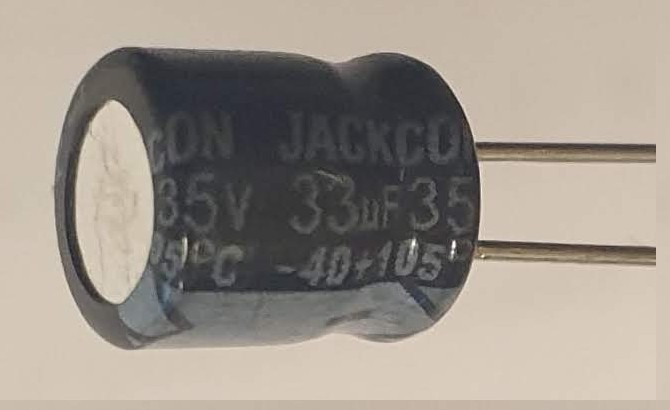
\includegraphics[width=.6\textwidth]{capa.jpg}
	\end{center}
}
{
	On voit son intervalle de températures acceptable : -40°C à +105°C, on pourrait donc le passer au four.
	Il s'agit d'un condensateur électrolytique, le temps se chargera de dégrader sa capacité.
	On voit aussi sa tension directe maximale : 35 V. C'est au-delà de ce dont sont capable l'alimentation du labo. On peut donc connecter une tension positive en inverse sur le condensateur (en pensant bien à ne pas limiter le courant de l'alim), à partir de 15 V ça claque.
	On peut aussi frapper dessus avec un marteau.
}


\section{Inspection et vérification d'un PCB}
L'assemblage d'un circuit imprimé est une tâche délicate.
Anticiper son comportement normal et le vérifier est donc essentiel et passe à nouveau par un protocole de test.

\Question{
	Choisissez un kit \text{Velleman} parmi ceux disponibles\footnote{S'il n'est pas encore assemblé, commencez par le monter.}.
	Inspectez sa documentation pour établir une \textbf{campagne} de test permettant de vérifier son bon fonctionnement.
	\begin{astuce}
	Une \textit{campagne} de test est constituée d'un ensemble de protocles de test.
	Chaque protocole se concentre sur une caractéristique particulière à vérifier, par exemple la présence de court-circuits dans le montage.
	\end{astuce}
}
{}



% \Question{
% 	Établissez un protocole vous permettant de vérifier qu'un condensateur électrolytique de 33 µF est en bon état.
% }
% {
% 	Inspection visuelle, vérification au multimètre ou au LCR, ou utilisation dans un montage.
% }

% \Question{
% 	Quelles sont les conditions de fonctionnement à ne pas dépasser pour votre condensateur ?
% }
% {
% 	Il s'agit généralement d'une tension positive à ne pas dépasser.
% }

% \Question{
% 	Quel est le moyen le plus efficace pour détruire ce condensateur ?
% }
% {
% 	La question est ouverte et on pourrait répondre « sauter dessus » ou « l'écraser avec un marteau ».
% 	La réponse découlant de la question précédente sera sans doute « en lui appliquant une tension plus grande que celle indiquée sur le condensateur. »
% 	Il est néanmoins possible de le détruire plus vite en lui appliquant une tension \textit{négative}, le condesateur électrolytique étant polarisé.
% }



% \section{Vérification d'un amplificateur opérationnel}
% Le \texttt{LM324} comprend quatre amplificateurs opérationnels dans le même boîtier.
% Les AOP utilisés en laboratoire n'étant pas toujours neufs, il est utile de pouvoir rapidement vérifier le bon fonctionnement du matériel avant de se lancer dans un montage complexe.

% \Question{
% 	Quelles sont les caractéristiques principales à vérifier ?
% }
% {
% 	Amplification correcte dans les bornes d'alimentation, produit gain$\cdot$bande passante.
% }

% \Question{
% 	Mettez en place un protocole de test permettant de vérifier qu'un \texttt{LM324} fonctionne correctement.
% }
% {
% 	Il faut en particulier faire attention aux alimentation et vérifier chaque AOP seul.
% 	Le protocole devrait proposer une méthode rapide pour tester chacun des quatre AOP et donc utiliser un montage simpliste.
% 	Si des résistances de rétroaction sont utilisées, elles devraient être connectées par des fils aux pattes de l'AOP de sorte qu'on doive simplement déplacer ces fils au cours du protocole, plutôt que déplacer les résistances elles-mêmes.

% 	Un montage suiveur ne nécessite aucune résistance et constitue un bon test initial. Il est cependant plus compliqué de vérifier le produit gain$\cdot$bande passante avec un gain de seulement 1.
% }


% \section{Condensateur}
% \begin{itemize}
% 	\item Transistor claqué. Les trouver parmi une pile de condensateurs masqués.
% 	\item Transistor claqué, savoir l'identifier visuellement.
% \end{itemize}


% \section{Transistor}
% \begin{itemize}
% 	\item Court-circuité.
% \end{itemize}

% \section{Résistance}
% \begin{itemize}
% 	\item Résistance cramée et noire.
% \end{itemize}



\end{document}
